\subsection{Training specifications}
We have talked about hyperparameters of the network that we need to tune, but there are also some specifications of the training, itself. These settings are used during the training on all of the models. 

\subsubsection{Early stopping algorithm}

The training process is observed by the early stopping algorithm, which stops the training after the validation loss is not improving for a certain period. However, after training several models we have noticed that the lowest validation loss for real data doesn't correspond to the highest accuracy. This may be due to some outliers in the validation set that increase the loss, even though the classification performs adequately. 

This phenomenon is shown in the Figure \ref{fig:esalossacc1}, where we show the progress of the validation loss and accuracy during the training of one of the models. You may notice that from a certain epoch the validation loss on the real data (orange line) starts to increase (Figure \ref{fig:loss1}) and the early stopping algorithm stops the training after some time. However, if we look at the progress of the accuracy (Figure \ref{fig:acc1}) we see that at that exact point (red dotted line) the accuracy starts to increase. The model should be trained for more epochs but since the early stopping algorithm stops the training, we can't achieve better accuracy. 

To prevent this problem we have decided to use accuracy instead of loss for the early stopping algorithm. Based on some observations, we have noticed that loss and accuracy on the synthetic validation set follow a similar path as accuracy and loss on the training set. For this reason, we are using accuracy on the real images in the validation set.  

The training will proceed for 100 epochs and stops if the validation accuracy doesn't improve after 10 epochs. This waiting time of 10 epochs is also referred to as a parameter patience. 

\begin{figure}[!h]
\centering
    \begin{subfigure}[t]{.45\textwidth}
        \centering
        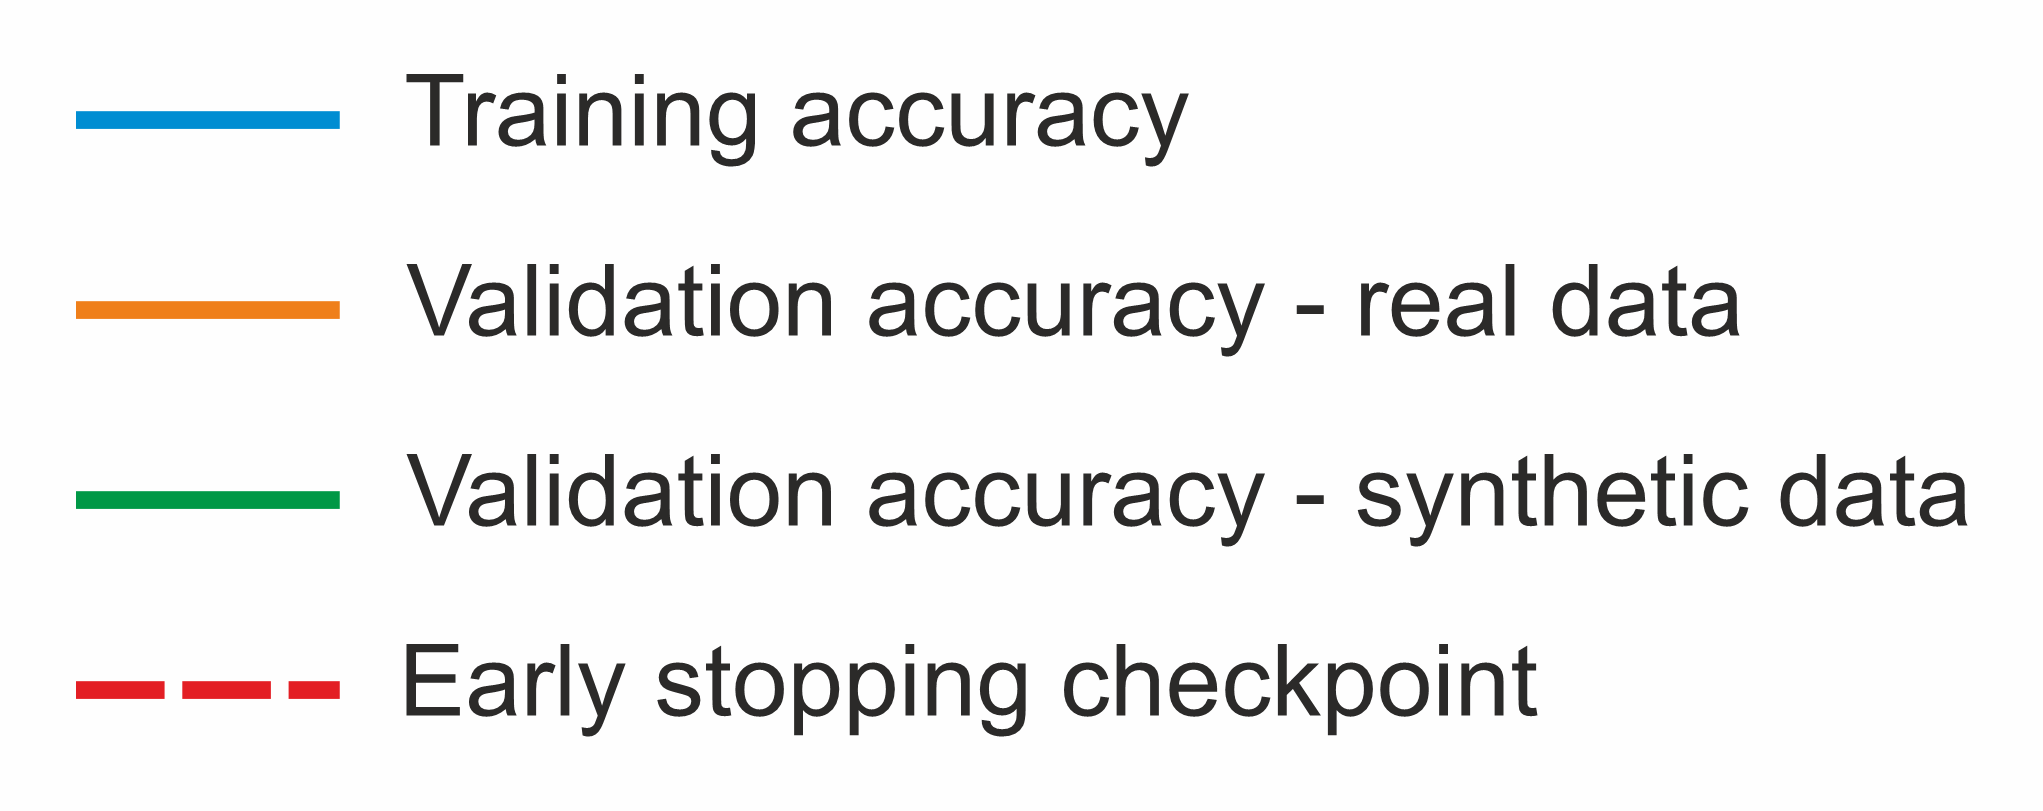
\includegraphics[width=.7\textwidth]{images/popisAc.png}
        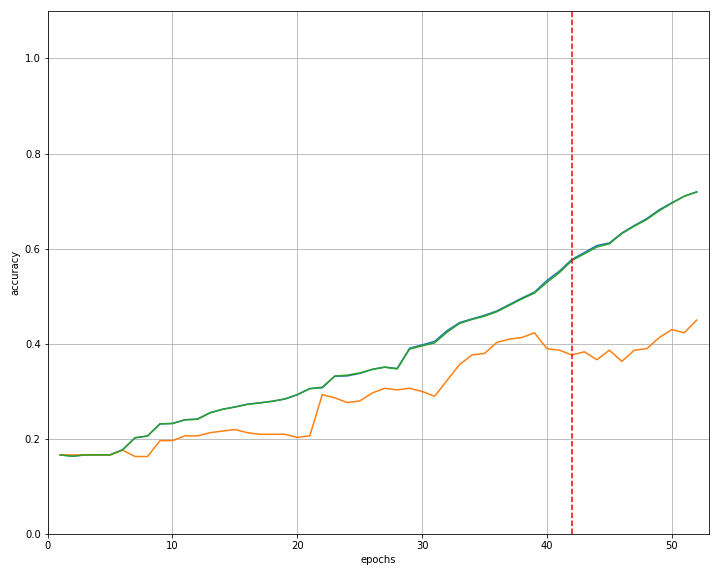
\includegraphics[width=\textwidth]{images/accuracy1ss_0.png}
        \caption{Evolution of the accuracy during training.}
        \label{fig:acc1}
    \end{subfigure}
    \begin{subfigure}[t]{.45\textwidth}
        \centering
        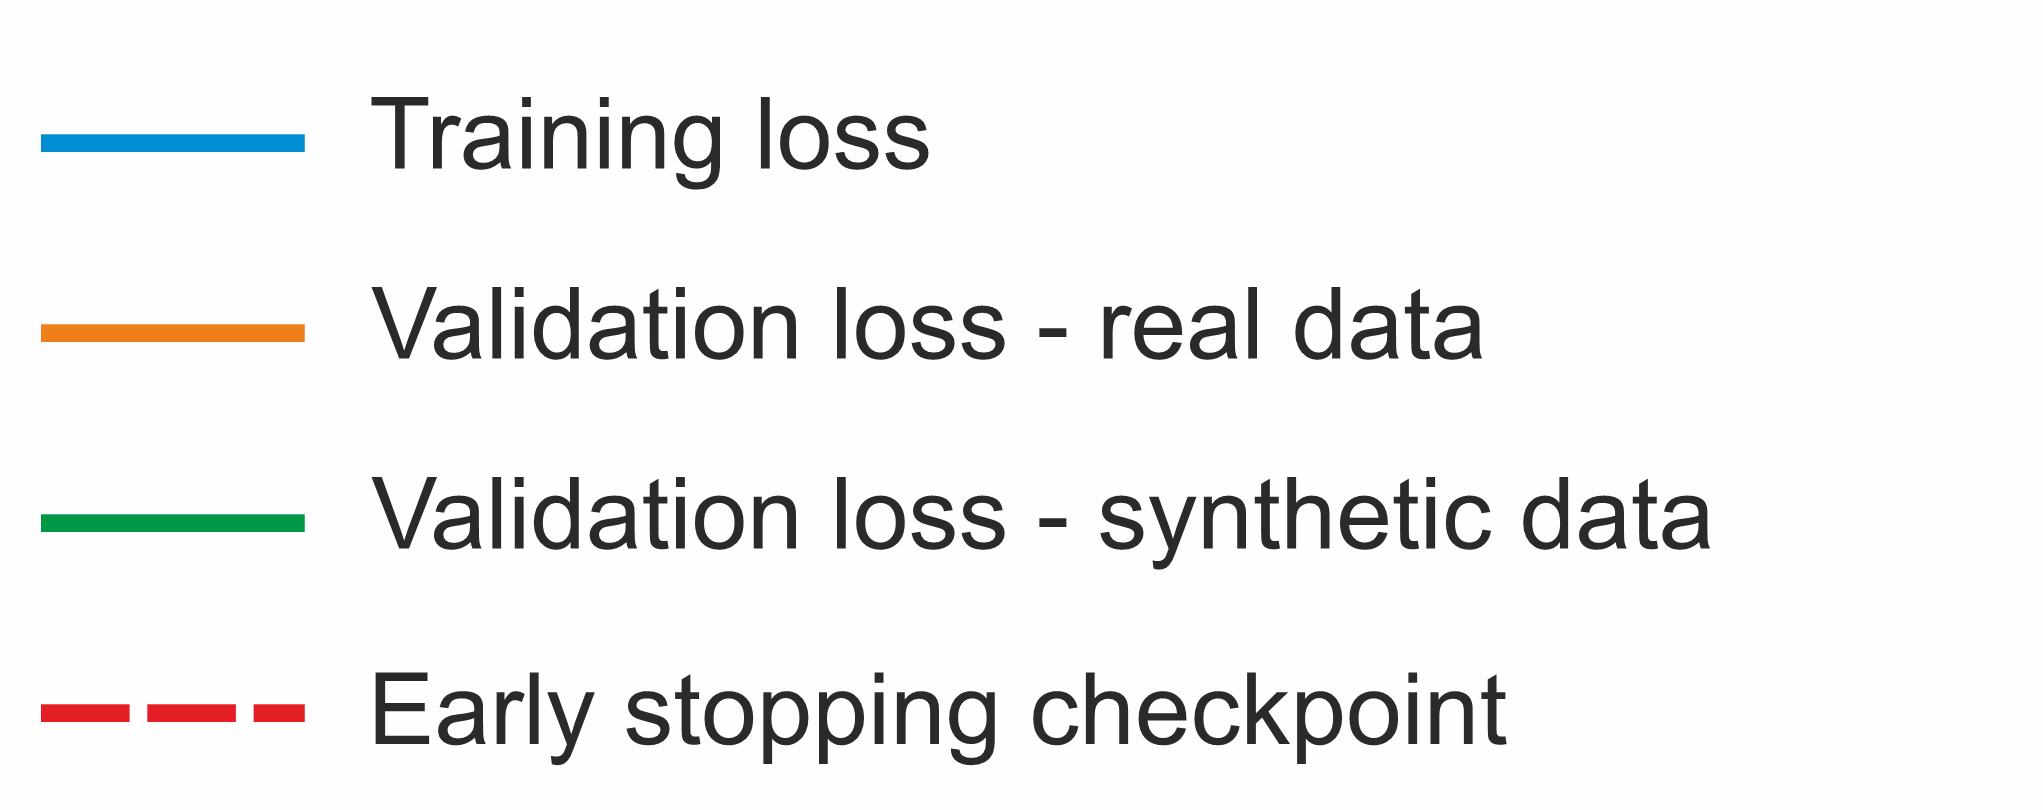
\includegraphics[width=.7\textwidth]{images/popisLoss.png}
        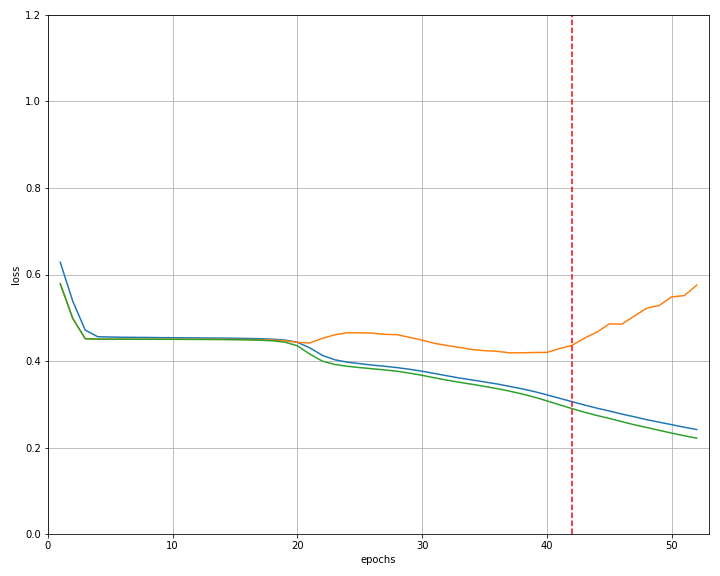
\includegraphics[width=\textwidth]{images/losses1ss_0.png}
        \caption{Evolution of the loss during training.}
        \label{fig:loss1}
    \end{subfigure}

    \caption{The increase of both the accuracy and the loss on the validation set of real images from a checkpoint.}
    \label{fig:esalossacc1}
\end{figure}


\subsubsection{Multiple models}

Training of the network also depends on some random operations like initial values of the weights or the division of images into batches. To avoid the randomness affecting our results, we train 10 models on each configuration of parameters. The provided metrics are then measured as average over all 10 models. 